Dans les disques radiatifs, la migration de type I est gouvernée par le couple différentiel de Lindblad, qui induit généralement
une migration vers l'intérieur \citep{tanaka2002three}, et le couple de corotation, qui peut contrebalancer le couple
différentiel de Lindblad sous certaines conditions et ainsi inverser le sens de migration (vers l'extérieur)
\citep{paardekooper2006halting, kley2008migration}. Il est donc possible d'avoir dans un disque des zones où la migration
s'arrête. Ces zones sont appelées zone de convergence \citep[CZs;][]{lyra2010orbital, mordasini2011application,
paardekooper2011torque}. 

\bigskip

À la zone de convergence, le couple de corotation (positif) compense exactement le couple différentiel de Lindblad (négatif).
Ainsi, à la zone de convergence, une planète ne migre pas.

De plus, autour de la zone de convergence, la migration tend à ramener les embryons vers la zone de couple nul s'ils s'en
éloignent. La zone de convergence est donc une position stable dans le disque vers laquelle les embryons se rassemblent.

Il peut exister de même des zones de couples nuls qui ne sont pas des zones de convergence quand, en s'éloignant légèrement, la
migration tend à les éloigner davantage. Ces zones sont alors instables.

Les zones de convergences pourraient ainsi concentrer les embryons planétaires et être le lieu de formation de planètes (ou
cœurs) massives \citep{lyra2010orbital, horn2012orbital}. 

\section{Disque de référence}\label{sec:migrations-maps}\label{sec:reference_disk}
%TODO parler des raisons pour lesquelles la zone de convergence dépend de la masse et de la distance parfois, avec les
%comparaisons des temps (dynamique, de U-turn and de diffusion)

\begin{figure}[htb]
\centering
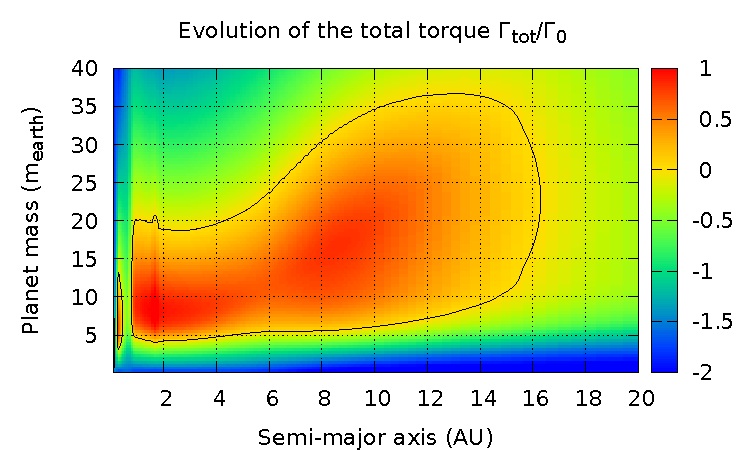
\includegraphics[width=\linewidth]{figure/migration_map/fiducial.pdf}

\caption{Carte de migration pour le disque fiducial. Cette carte montre le sens de migration d'une planète en fonction de sa
position (abscisse) et de sa masse (ordonnée). La 3\ieme coordonnée est le couple total exercé par le disque sur la planète,
exprimé en unité de $\Gamma_0 = \left(\frac{q}{h}\right)^2\Sigma_p {r_p}^4 {\Omega_p}^2$. Quand le couple est positif (resp.
négatif), la migration est vers l'extérieur (resp. intérieur). La ligne noire représente la zone de couple nul, où la planète ne
migre plus. Le détail des paramètres du disque de référence est donné \reftab{tab:fiducial_parameters}.
}\label{fig:fiducial_migration_map}
\end{figure}

Dans cette section, nous allons présenter notre disque de référence et comment ses paramètres vont influencer la migration des
planètes. Ce disque de référence servira aussi de comparaison quand nous étudierons les effets des paramètres du disque.

Afin d'étudier la migration dans les disques, il est pratique de regarder une \og carte de migration\fg, comme
\reffig{fig:fiducial_migration_map}. Cette carte permet de voir rapidement les parties intéressantes et de prédire l'évolution
d'une planète à partir de la position et masse initiales.

\reffig{fig:fiducial_migration_map} montre la carte de migration du disque de référence que nous utiliserons de manière
récurrente ici. Ce disque est obtenu à l'aide de la table d'opacité d'\cite{hure2000transition}. Le profil de température est
calculé en tenant compte de l'irradiation, avec des paramètres solaires pour la température et le rayon de l'étoile ($T_\star =
5700\unit{K}$ ; $R_\star = 4.65\cdot 10^{-3}\unit{AU}$). L'albédo du disque est pris égal à $0.5$. La viscosité est calculée à
partir d'une prescription alpha \citep{shakura1973black}. On considère un disque dont les bords internes et externes sont
respectivement à $0.1$ et $100\unit{UA}$. Les autres paramètres du disques sont récapitulés \reftab{tab:fiducial_parameters}. 

\begin{table}[htb]
\centering
\begin{tabular}{|c|c|c|c|}
\hline
$b/h = 0.4$ & $\gamma = 7/5$ & $\mu = 2.35$ & $\alpha = 5\cdot 10^{-3}$ \\\hline
\multicolumn{2}{|c|}{Inner edge : $0.1\unit{UA}$} & \multicolumn{2}{c|}{Outer edge : $100\unit{UA}$}\\\hline
\multicolumn{4}{|c|}{$\Sigma(R) = 300 \cdot R^{-1/2}\unit{g/cm^2}$}\\\hline
$T_\star = 5700\unit{K}$ & $R_\star = 4.65\cdot 10^{-3}\unit{AU}$ & \multicolumn{2}{c|}{Disk albedo : $0.5$}\\\hline
\end{tabular}
\caption{Paramètres physiques du disque fiducial. Les opacités sont calculées à partir de la table d'opacité de
\cite{hure2000transition}. La viscosité est calculée en suivant la prescription alpha de
\cite{shakura1973black}.}\label{tab:fiducial_parameters}
\end{table}

\begin{figure}[htb]
\centering
\subfloat[Lindblad torque]{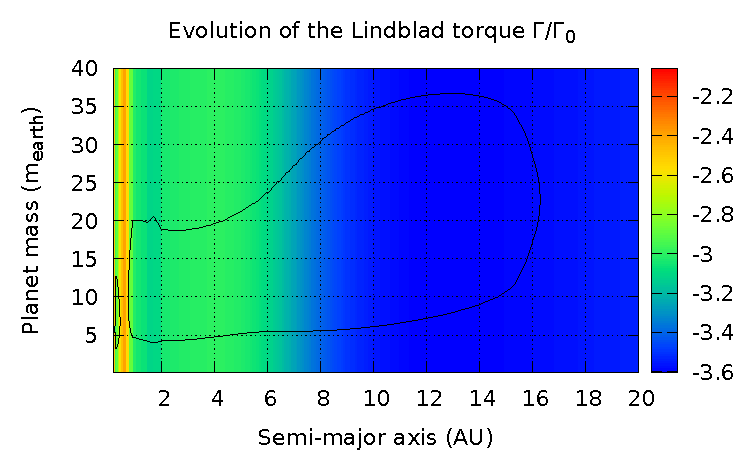
\includegraphics[width=0.49\textwidth]{figure/migration_map/details/lindblad_torque.pdf}}\hfill
\subfloat[Horseshoe Entropy related torque]{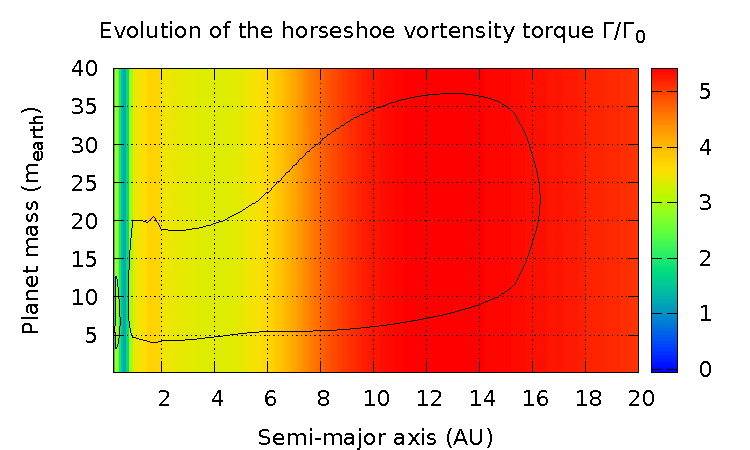
\includegraphics[width=0.49\textwidth]{%
figure/migration_map/details/ent_hs_torque.pdf}}

\caption{Evolution des deux couples les plus importants vis à vis de la carte de migration, le couple de Lindblad et la partie
non saturée du couple de corotation liée au gradient d'entropie. En effet, ces deux couples sont quantitativement plus grand que
tous les autres. Ici, seule la partie non-saturée du couple de corotation est représentée.}\label{fig:details_maps}
\end{figure}

Sur \reffig{fig:details_maps} sont représentés les deux couples les plus importants en terme d'amplitude (tant négative pour le
couple de Lindblad $\Gamma_L$, que positive pour la partie du couple de corotation non saturée liée au gradient d'entropie
$\Gamma_\text{ent,hs}$. Ici, c'est bien la partie non saturée qui est représentée \og fully unsaturated\fg. On ne tiens pas
compte de la diffusion. On constate alors que sans tenir compte de la diffusion, les couples sont totalement indépendants de la
masse. La transition que l'on constate dans les deux cartes, entre $6-8\unit{UA}$ correspond à la transition disque
actif/passif. L'irradiation est le processus de chauffage principal à partir de $5\unit{UA}$ comme illustré par
\reffig{fig:viscous_vs_irradiation}.

\begin{figure}[htb]
\centering
\subfloat[$t_\text{rad}/t_\text{U-turn}$]{\label{fig:linear_rad}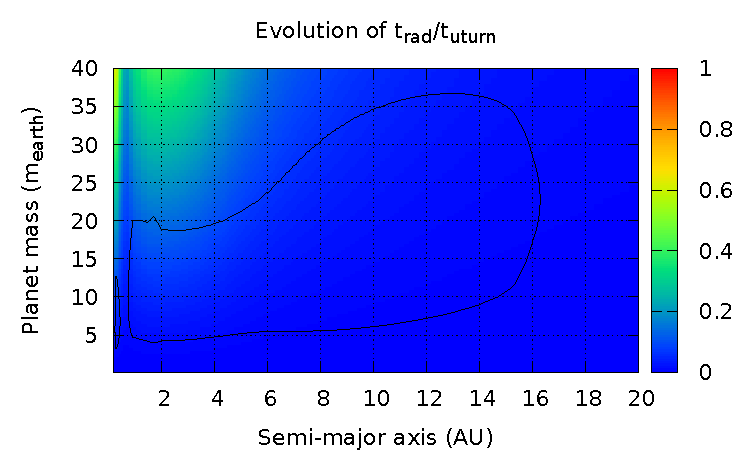
\includegraphics[width=0.49\textwidth]{%
figure/timescales/linear_rad.pdf}}\hfill
\subfloat[$(t_\text{lib}/2)/t_\text{visc}$]{\label{fig:sat_visc}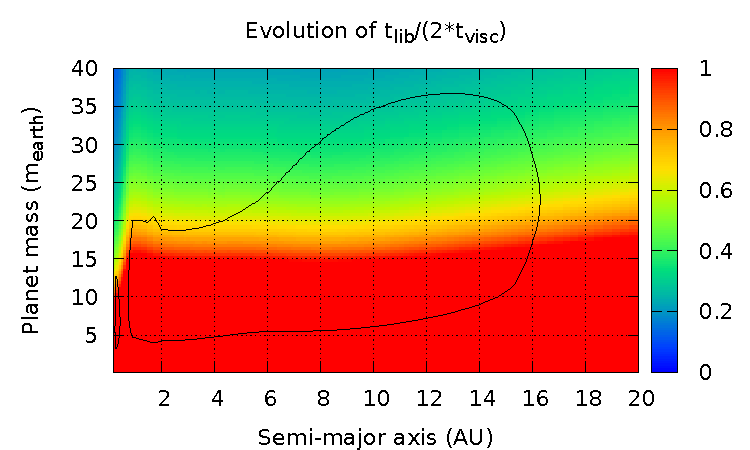
\includegraphics[width=0.49\textwidth]{%
figure/timescales/sat_visc.pdf}}

\caption{Comparaison des différents temps caractéristiques influençant le couple de corotation. Ces inéquations sont détaillées
dans \refsec{sec:couple-corotation}. Dans le cas présent, le temps de diffusion radiative est toujours plus court que le temps
de diffusion visqueuse, $t_\text{rad}<t_\text{visc}$. Ainsi il ne reste plus que les deux inégalités représentées
ici.}\label{fig:timescales_maps}
\end{figure}

\reffig{fig:timescales_maps} représente l'effet de la diffusion sur la carte de migration. Seuls deux cartes sont montrées,
contrairement aux quatres que nous pourrions attendre, car $t_\text{rad}<t_\text{visc}$. Ainsi, la double inégalité, qui était
scindable en 4 sous-inégalités (deux pour chaque temps de diffusion) devient :
\begin{align}
t_\text{U-turn} < t_\text{diff} < \frac{t_\text{lib}}{2}\\
t_\text{U-turn} < t_\text{rad} < t_\text{visc} < \frac{t_\text{lib}}{2}
\end{align}

À partir de \reffig{fig:timescales_maps} on constate deux choses. La première c'est que la zone de couple nul du bas de la carte
de migration, est régie par l'inéquation $t_\text{U-turn} < t_\text{rad}$ \reffig{fig:linear_rad}. C'est surtout visible dans la
partie $0-4\unit{UA}$ où l'irradiation ne domine pas encore le profil de température. En dessous de cette ligne, c'est
uniquement la partie linéaire du couple de corotation qui subsiste. Le temps de diffusion radiatif $t_\text{rad}$ est trop court
pour que la zone fer-à-cheval induise une variation des propriétés du disque lors du demi-tour devant la planète. 

La partie supérieure de la carte, quant à elle, est due à la saturation du couple de corotation, illustrée par l'inégalité
$(t_\text{lib}/2) > t_\text{visc}$ qui doit être vérifiée pour que le couple ne sature pas \reffig{fig:sat_visc}. Comme
précédemment, au delà de $4\unit{UA}$ l'irradiation domine peu à peu le bilan énergétique du disque, et dilate la zone en masse
pour laquelle une planète ressens un couple positif.

\begin{figure}[htb]
\centering
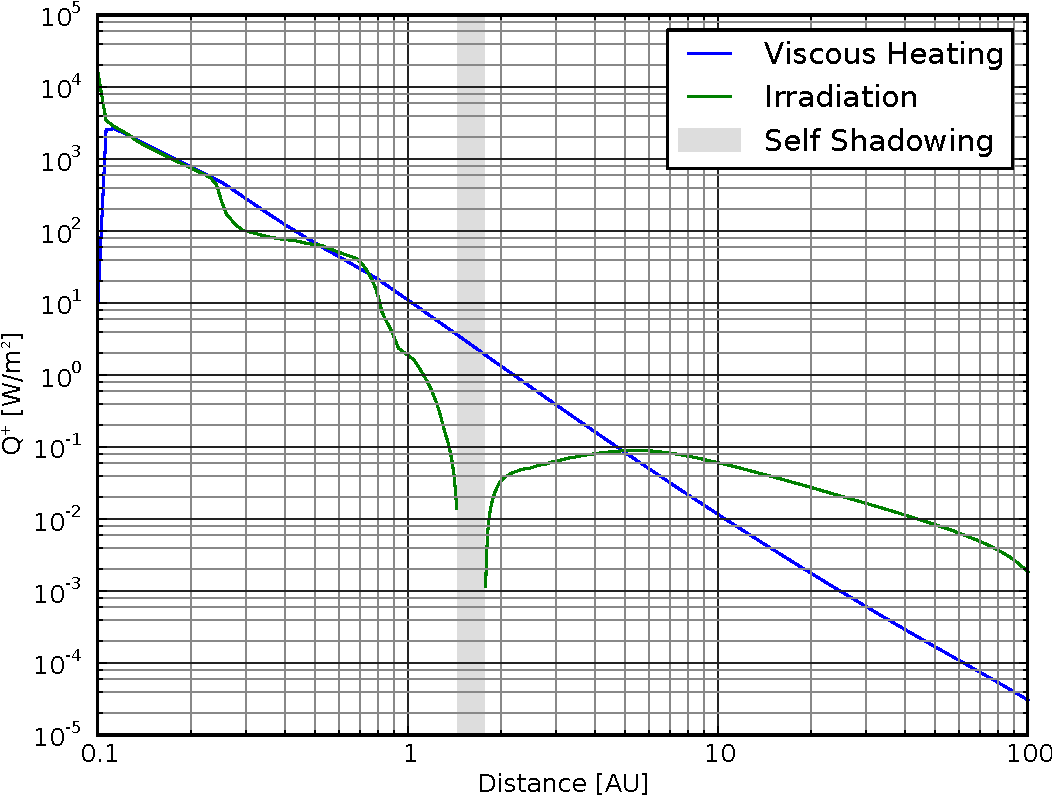
\includegraphics[width=0.75\textwidth]{figure/migration_map/viscous_vs_irradiation.pdf}

\caption{Évolution du chauffage visqueux et de l'irradiation en fonction de la distance. Dans les parties internes, c'est le
chauffage visqueux qui domine. Dans les parties externes c'est l'irradiation. À $5\unit{UA}$ les deux contributions sont
équivalents.}\label{fig:viscous_vs_irradiation}
\end{figure}

\reffig{fig:viscous_vs_irradiation} montre qu'au delà de $5\unit{UA}$ l'irradiation domine le bilan énergétique du disque. Cela
correspond à la distance à laquelle les cartes mettant en jeu les temps de diffusions n'expliquent plus la forme de la carte de
migration. À partir de cette distance là, l'irradiation dilate la carte de migration

Intéressons nous maintenant aux zones qui ferment verticalement les lignes de couple nul. Dans les parties externes, après
$15\unit{UA}$, c'est la conjonction des deux processus de diffusion qui \og ferme\fg le profil de couple. Pour les masses
faibles, en dessous de $15-20\mearth$, la migration vers l'intérieur est dur au fait que $t_\text{U-turn} > t_\text{rad}$, c'est
alors la valeur linéaire du couple de corotation qui prévaut. Pour les masses plus importantes, le couple de corotation sature
car $(t_\text{lib}/2) < t_\text{visc}$. 

Avant $1\unit{UA}$, les deux régions de couples positifs sont séparés. C'est une transition d'opacité à $1\unit{UA}$ environ qui
en est la cause, et qui change brusquement les couples de migration, quelle que soit leur origine \reffig{fig:details_maps}. Ce
brusque changement d'opacité et de température est la raison de la séparation de la zone de couple positif en deux. Ainsi, les
raisons valables à $15\unit{UA}$ le sont ici aussi, mais la variation du couple en fonction de la distance est beaucoup plus
grande, de sorte que la position de la zone de convergence semble ne pas dépendre de la masse, contrairement aux parties
externes de la carte de migration.

\section{Différents types de zone de convergence}\label{sec:CZ-types}
En fonction de la distance, nous pouvons définir des masses critiques extrémales au delà desquelles la migration vers
l'extérieur est impossible en raison du temps de diffusion qui est soit trop grand (saturation) soit trop petit (couple
linéaire) pour qu'un couple de corotation non saturé puisse exister.

Mais l'information la plus importante de ces cartes de migration est certainement l'évolution du couple en fonction de la
distance. Nous pouvons dégager deux types particulier de zones de convergence. 

Le premier type de zone de convergence est ce que nous appellerons une zone de convergence indépendante de la masse. C'est une
zone qui se trouve plutôt dans les parties interne du disque. Cette ligne de couple nul dépend très peu de la masse de la
planète car une transition d'opacité induit de brusques changements de température. Les couples varient ainsi fortement sur une
distance très courte. Cette zone de convergence a deux caractéristiques importantes : 
\begin{enumerate}
\item La position de la zone de convergence ne dépend pas ou peu de la masse de planète
\item La variation du couple de migration autour de la zone de convergence est très forte
\end{enumerate}

Nous pouvons appeler le deuxième type \og zone de convergence dépendant de la masse\fg. En effet, dans les parties externes, le
couple varie plus doucement en fonction de la distance. L'influence de la masse est donc plus marqué dans la position de la zone
de couple nul. Ce type de zone de convergence a deux caractéristiques importantes : 
\begin{enumerate}
\item La position de la zone de convergence dépend de la masse de la planète. 
\item Le couple de migration varie doucement en fonction de la distance à la zone de convergence
\end{enumerate}

\begin{figure}[htb]
\centering
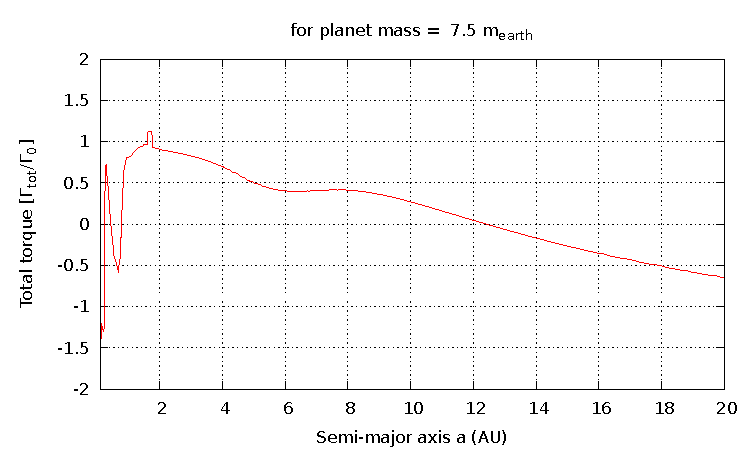
\includegraphics[width=0.75\linewidth]{figure/total_torque_fixed_m.pdf}
\caption{Évolution du couple total exercé par le disque sur une planète de $7.5\mearth$. }\label{fig:total_torque_fixed_m}
\end{figure}

\reffig{fig:total_torque_fixed_m} illustre les deux zones de convergences. La première près de $1\unit{UA}$, siège d'une
variation brutale du couple de migration, et la deuxième (dont la position dépend de la masse de la planète) où la variation du
couple de migration est continue. 

Dans la suite, nous avons parfois utilisé des zones de convergences artificielles afin de simplifier les effets, et d'étudier
plus facilement un phénomène particulier. Dans le cas d'une transition d'opacité, nous avons modélisé les zones de convergence
indépendantes de la masse par une tangente hyperbolique dont le zéro se situe à la zone de convergence, et où le couple de
migration (positif ou négatif) sature très loin de la zone de convergence \refsec{sec:tanh_indep}. Pour modéliser une zone de
convergence indépendante de la masse où le couple varie peu autour de la zone de convergence, nous avons utilisé une variation
linéaire du couple de migration \refsec{sec:linear_indep}.

Les zones de convergence dépendantes de la masse peuvent être approximées par une variation linéaire de la position de la zone
de couple nul en fonction de la masse. Le couple de migration varie quant à lui linéairement en fonction de la distance
\refsec{sec:mass_dependant}. 



\section{Effets des paramètres du disque}
%TODO see kretke2012importance
%TODO regarder le papier de Bitsch 2013 et celui de 2012 où il regarde l'influence de l'indice adiabatique
%TODO essayer des gammes beaucoup plus larges de paramètres

Jusqu'à présent, je me suis concentré sur des cas particuliers. Dans le cas de la formation de super-Terres, je n'ai considéré
qu'un seul disque \refsec{sec:4.2}. Dans le cas du décalage de la zone de convergence, j'ai montré un disque artificiel
modélisant une zone de convergence \refsec{sec:shifted_CZ}. 

Je vais montrer dans les paragraphes qui suivent que la migration est extrêmement sensible aux paramètres du disque.

\cite{kretke2012importance} ont étudié l'influence des paramètres du disque sur la migration. Cependant, s'ils ont inclus des
effets fins sur le bord interne et la migration, la dépendance de l'opacité en fonction de la température et de la densité est
approximée par différentes lois de puissance. Nous montrerons que l'opacité est un paramètre sensible du modèle et qu'il est
important de la modéliser le plus finement possible. 

\cite{bitsch2013influence} ont étudié en particulier l'effet de la viscosité $\nu$ et l'indice adiabatique $\gamma$ sur la
migration dans le disque, au travers de simulations 3D. 

Afin d'étudier séparément l'effet des paramètres du disque, j'ai choisi un disque de référence, décrit
\refsec{sec:migrations-maps}. Dans cette section je présente les cartes de migration et comment les interpréter. En particulier
je présente la carte de migration du disque de référence \reffig{fig:fiducial_migration_map}. Pour chaque paramètre, je vais
donc conserver les valeurs du disque fiducial, et faire varier le paramètre en question autour de la valeur de référence. Sauf
mention contraire, un seul paramètre est donc modifié à la fois, seuls les paramètres qui changent sont précisés, les autres
sont regroupés \reftab{tab:fiducial_parameters}.

%TODO continuer

%TODO 
\subsection{Viscosité du disque}

%TODO 

Le couple de migration est sensible à la valeur de la viscosité $\nu$. En particulier, c'est l'efficacité de la diffusion
visqueuse qui modifie le niveau de saturation du couple de corotation. 

\begin{figure}[htb]
\centering
\subfloat[$\alpha=5.10^{-3}$]{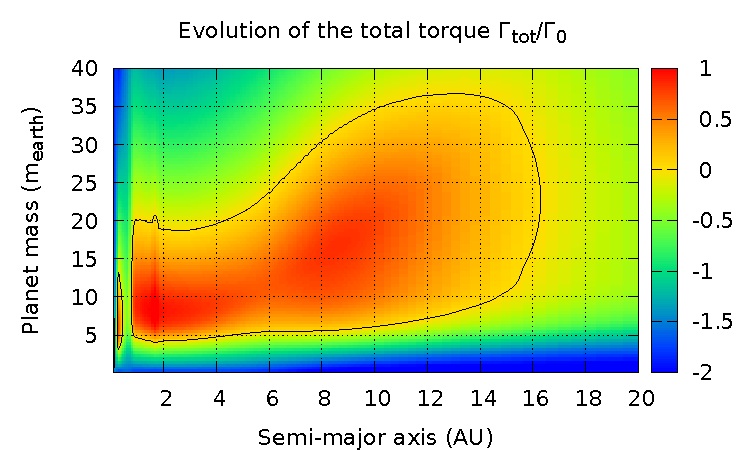
\includegraphics[width=0.49\textwidth]{figure/migration_map/viscosity/alpha.pdf}}\hfill
\subfloat[$\alpha=5.10^{-3}$ + dead zone]{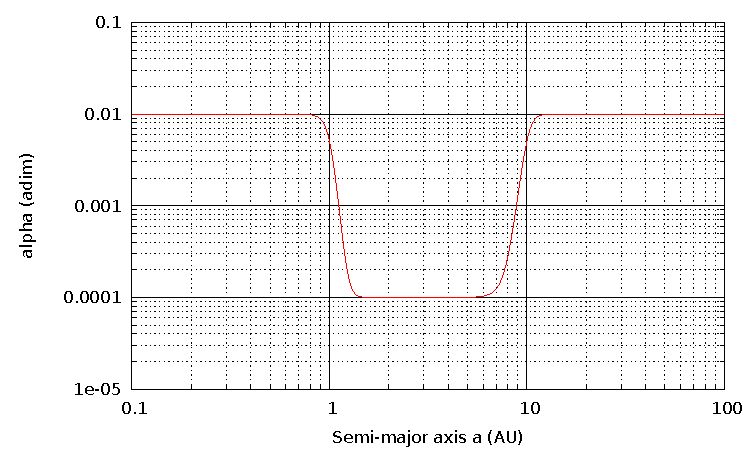
\includegraphics[width=0.49\textwidth]{%
figure/migration_map/viscosity/alpha_dz.pdf}}

\subfloat[$\nu=10^{14}\unit{cm^2/s}$]{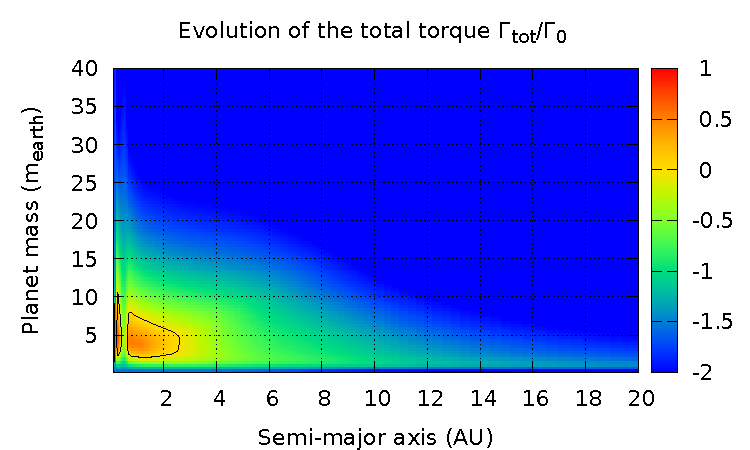
\includegraphics[width=0.49\textwidth]{figure/migration_map/viscosity/constant_1e14.pdf}}
\hfill
\subfloat[$\nu=10^{15}\unit{cm^2/s}$]{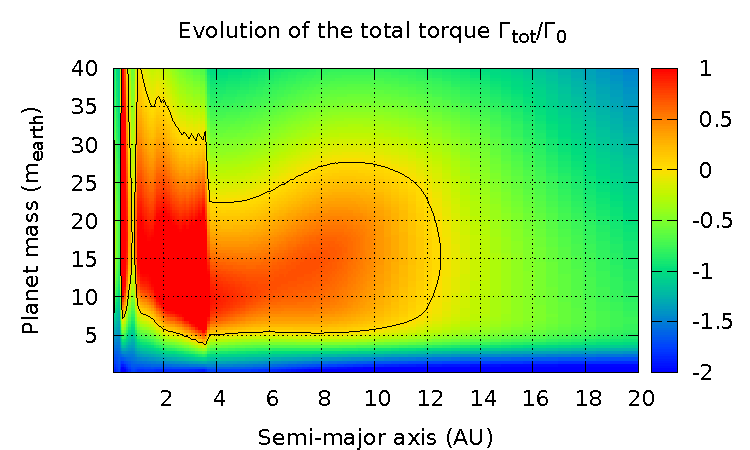
\includegraphics[width=0.49\textwidth]{%
figure/migration_map/viscosity/constant_1e15.pdf}}
\caption{Cartes de migration obtenues pour le disque de référence \protect\reffig{fig:fiducial_migration_map} dans lequel on ne
modifie que la viscosité. Dans la première carte, la viscosité est régie par un modèle alpha où $\alpha=5.10^{-3}$ (ce qui est
utilisé dans le disque de référence). Dans la deuxième carte, on rajoute en plus une zone morte où la valeur de alpha est plus
faible $\alpha=10^{-4}$. Plus de détails sur la modélisation de la zone morte \protect\refsec{sec:dead_zone}. Enfin, deux
modèles à viscosité constante $\nu=10^{14}\unit{cm^2/s}$ et $\nu=10^{15}\unit{cm^2/s}$ sont aussi représentés. \refdisk}
\end{figure}\label{fig:viscosity_comparison}

Pourtant, la carte de migration possède une deuxième sensibilité au modèle de viscosité. Selon que l'on choisi une viscosité
constante ou une prescription alpha dans laquelle la viscosité $\nu$ croit avec la distance, cela a une influence sur
l'évolution du couple en fonction de la position dans le disque. 

\begin{figure}[htb]
\centering
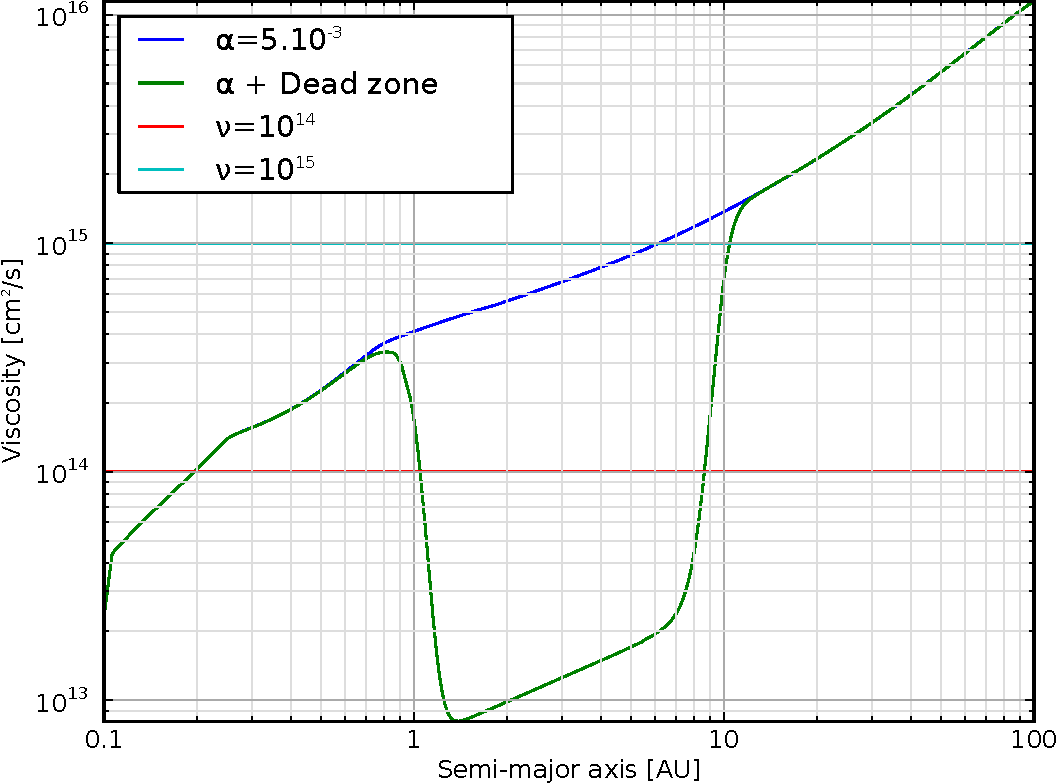
\includegraphics[width=0.6\linewidth]{figure/migration_map/viscosity_profile.pdf}
\caption{Profils de viscosité du disque en fonction des modèles, deux où la viscosité est constante, un avec une viscosité
alpha, et un dernier qui modélise en plus une zone morte. Ces profils correspondent à chacune des quatres cartes de migration
présentées Figure~\ref{fig:viscosity_comparison}. \refdisk}\label{fig:viscosity_profiles}
\end{figure}

Avec un modèle alpha $\alpha=5.10^{-3}$, la viscosité à $0.2\unit{UA}$ est $\nu=10^{14}\unit{cm^2/s}$, tandis qu'elle est de
$\nu=10^{15}\unit{cm^2/s}$ à $6\unit{UA}$. Les deux modèles à viscosité constante permettent donc de voir à quoi ressemblait la
carte de migration si c'était la viscosité au bord ou au milieu du disque qui était prise comme référence. En effet, dans le
modèle alpha, la viscosité varie de plusieurs ordres de grandeur, depuis $\nu=3.10^{13}\unit{cm^2/s}$ au bord interne
($0.1\unit{UA}$) jusqu'à $\nu=10^{16}\unit{cm^2/s}$ au bord externe ($100\unit{UA}$).

\subsection{Masse du disque}
%TODO discuter la dissipation plus en détail, en particulier reprendre la partie dissipation phtooévaporation du début, et
%discuter de ce qu'il pourrait se passer au niveau de la migration par rapport à ce que j'ai extrait des effets du disque.
\begin{figure}[htb]
\centering
\subfloat[$\Sigma_0=400\unit{g/cm^2}$]{\label{fig:map_low_mass}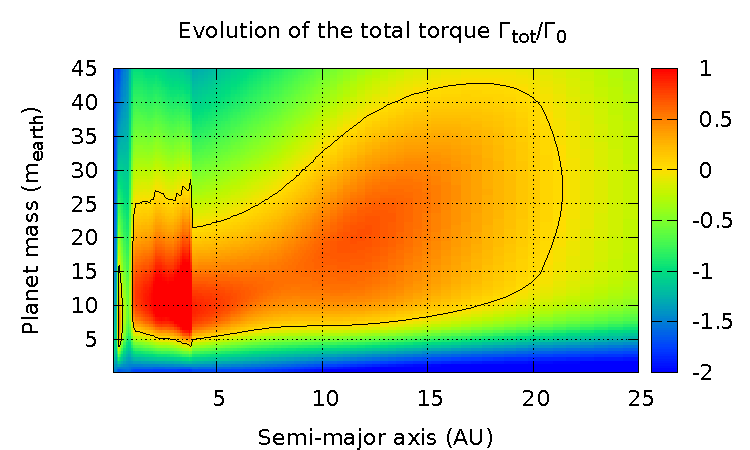
\includegraphics[width=0.49\textwidth]{%
figure/migration_map/total_mass/high_mass.pdf}}\hfill
\subfloat[$\Sigma_0=200\unit{g/cm^2}$]{\label{fig:map_high_mass}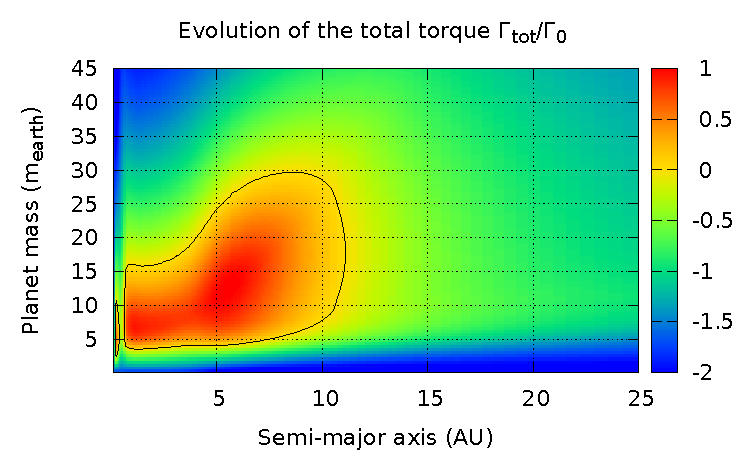
\includegraphics[width=0.49\textwidth]{%
figure/migration_map/total_mass/low_mass.pdf}}

\caption{Par rapport au disque de référence, possédant un profil de densité de surface $\Sigma(R) = 300 \cdot
R^{-\sfrac{1}{2}}\unit{g/cm^2}$ nous représentons la carte de migration dans un cas un peu moins et un peu plus massif, avec le
même indice de la loi de puissance. Les échelles ne sont pas les mêmes, elles ont été choisies pour montrer que la forme reste
globalement conservée, si on s'affranchi de l'échelle absolue de la taille de cette dernière.
\refdisk}\label{fig:map_total_mass}
\end{figure}

Dissiper le disque par une exponentielle décroissante signifie changer la masse du disque au cours du temps sans modifier
l'indice $d$ de la loi de puissance pour la densité de surface.

Pendant la dissipation, la zone de convergence externe va peu à peu se déplacer vers l'intérieur du disque. La zone de
convergence externe qui était à $20\unit{UA}$ environ pour des planètes dont la masse est comprise entre $15$ et $40\mearth$
\reffig{fig:map_high_mass} va se retrouver à $10\unit{UA}$ environ avec un disque moins massif \reffig{fig:map_low_mass}. 

À partir de la carte de migration d'un disque donné nous pouvons définir la masse critique supérieure (resp. inférieur) au
dessus (resp. en dessous) de laquelle on a systématiquement migration vers l'intérieur des planètes, quelle que soit leur
position. À mesure que le disque se dissipe,  les masses critiques diminuent. Ainsi, les planètes entre $30$ et $45\mearth$ qui
pouvaient auparavant migrer vers l'extérieur dans certaines zones du disque \reffig{fig:map_high_mass} ne peuvent plus le faire
dans un disque un peu moins massif \reffig{fig:map_low_mass}. Les planètes entre $3$ et $5\mearth$ qui ne pouvaient que migrer
vers l'intérieur \reffig{fig:map_high_mass} peuvent maintenant migrer vers l'extérieur dans certaines zones du disque moins
massif \reffig{fig:map_low_mass}. 

On pourrait penser que cette étude de l'influence de la masse du disque sur la carte de migration nous permet de comprendre
l'influence de la dissipation du disque sur la migration. Il n'y a rien de plus faux. En particulier la deuxième phase de la
dissipation du disque, rapide et que l'on pense due à la photoévaporation n'est pas uniforme. Elle ne conserve pas la pente
d'une loi de puissance, si tant est qu'on puisse définir le profil original en terme de loi de puissance. Au lieu de ça, le
disque va se creuser à partir d'un certain rayon, optimal vis à vis de la photoévaporation. Ce dernier va alors se scinder en
deux, la partie interne va rapidement tomber sur l'étoile centrale et dans un dernier stade les parties externes vont aussi se
dissiper. Si les détails de la dissipation ne sont pas connus, il est clair qu'on ne peut pas considérer une
dissipation exponentielle pour toutes les phases de la dissipation. La modification du profil radial va avoir une importance
cruciale sur la 
dissipation d'une part, et sur la migration et la survie des planètes d'autre part. 

La dispersion du disque a été discutée brièvement \refsec{sec:dispersion}.

\subsection{Profil de densité de surface}
Dans notre modèle, le profil de la densité de surface est notre plus grande incertitude. Les contraintes observationnelles ne
restreignent pas suffisamment le profil de densité \citep[Fig. 12]{guilloteau2011dual}. Il y a peu de chance que la densité de
surface d'un disque réel puisse être défini par une loi de puissance d'un bout à l'autre, et surtout par la même loi de
puissance. 

On définit la loi de puissance pour la densité de surface de la façon suivante : 
\begin{align}
\Sigma(R) &= \Sigma_0 * \left(\frac{R}{R_0}\right)^{-d}
\end{align}
où $\Sigma_0$ est la densité de surface à $R_0=1\unit{UA}$.

Je cherche à étudier l'influence de l'indice $d$ de la loi de puissance sur la carte de migration. Je vais me concentrer sur
deux cas particuliers. Dans le premier cas, je vais étudier la variation de l'indice sans changer $\Sigma_0$, c'est à dire que
la masse totale du disque va varier en même temps que l'indice. Dans un deuxième cas, la masse totale du disque entre $0.1$ et
$100\unit{UA}$ est constante, et on varie la densité de surface à $1\unit{UA}$, $\Sigma_0$ en même temps que l'indice $d$ de la
loi de puissance.

\begin{figure}[htb]
\centering
\subfloat[$d=0.6$ ; $\Sigma_0=300\unit{g/cm^2}$]{\label{fig:d06}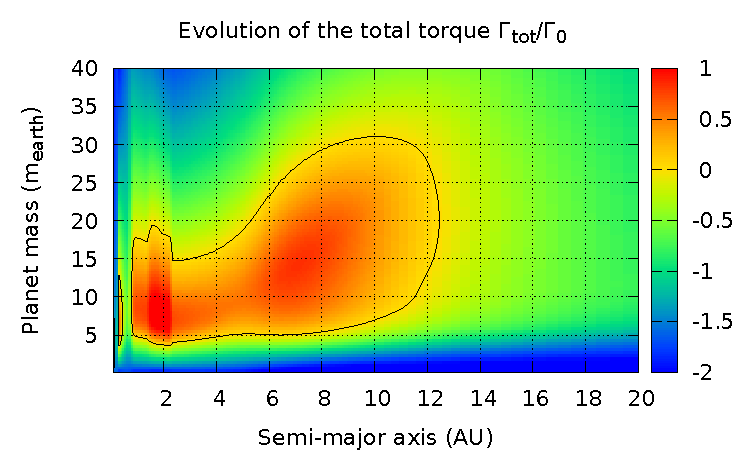
\includegraphics[width=0.49\textwidth]{%
figure/migration_map/index/300_06.pdf}}\hfill
\subfloat[$d=0.7$ ;
$\Sigma_0=300\unit{g/cm^2}$]{\label{fig:d07}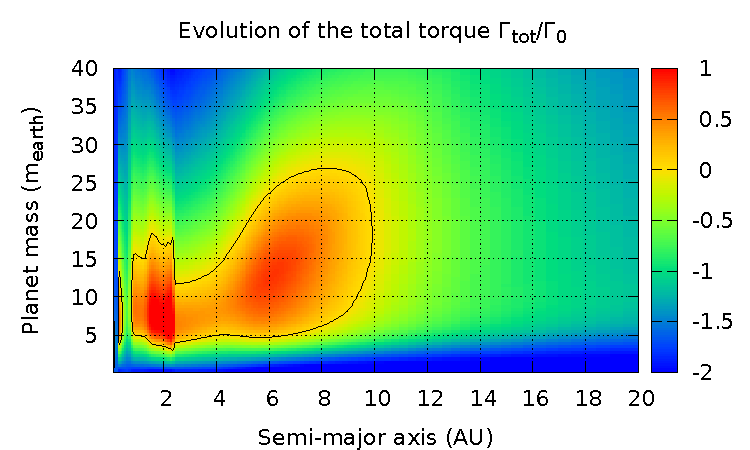
\includegraphics[width=0.49\textwidth]{figure/migration_map/index/300_07.pdf}}

\caption{Influence de l'indice $d$ de la loi de puissance définissant la densité de surface du disque sur la carte de migration.
Ici, $\Sigma_0=\cte=300\unit{g/cm^2}$, seul l'indice du profil de densité de surface varie. \refdisk}\label{fig:map_index}
\end{figure}

Si l'indice $d$ du profil de densité de surface augmente, la forme de la carte de migration aura tendance à se compresser vers
les parties internes du disque. En effet, en dessous de $R_0=1\unit{UA}$ la densité de surface sera plus importante si $d$
augmente. Mais dans les parties externes, au delà de $R_0=1\unit{UA}$ la densité de surface sera plus faible. La température
dans ces régions là sera alors plus faible. La diffusivité thermique $\chi$ étant extrêmement sensible à la température, si $T$
diminue cela entraine la diminution de $\chi$. Le temps de diffusion radiatif $t_\text{rad}$ étant inversement proportionnel à
la diffusivité thermique $\chi$, si l'indice du profil de densité de surface augmente, le temps de diffusion radiatif augmente.
En fonction de la distance, le couple de corotation sature ainsi plus rapidement. L'augmentation de $d$ dans
\reffig{fig:map_index} illustre cet aspect. 

On peut remarquer que l'augmentation de l'indice du profil de densité de surface va avoir un impact sur la masse totale du
disque. On a vu précédemment que la masse totale du disque avait un effet inverse par rapport à l'indice $d$. Si on augmente
l'indice $d$, on compresse la zone de migration externe vers l'étoile centrale. Au contraire, si on augmente la masse totale, on
dilate cette zone radialement. 

\begin{figure}[htb]
\centering
\subfloat[$d=0.6$ ; $\Sigma_0=444\unit{g/cm^2}$]{\label{fig:d06iso}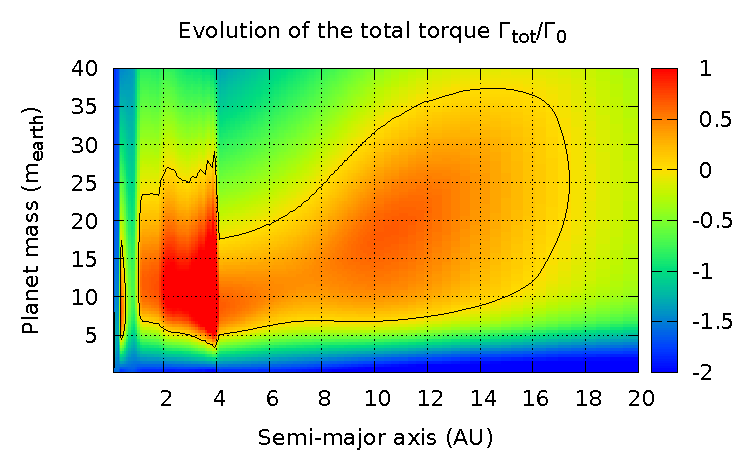
\includegraphics[width=0.49\textwidth]{%
figure/migration_map/index/444_06.pdf}}\hfill
\subfloat[$d=0.7$ ;
$\Sigma_0=653\unit{g/cm^2}$]{\label{fig:d07iso}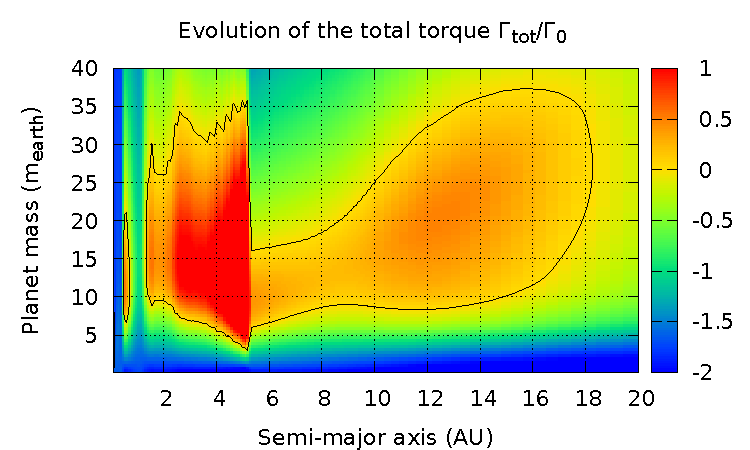
\includegraphics[width=0.49\textwidth]{figure/migration_map/index/653_07.pdf}}

\caption{Influence de l'indice $d$ du profil de densité de surface tout en maintenant la masse totale du disque constante.
\refdisk}\label{fig:map_index_mtot}
\end{figure}

On constate sur \reffig{fig:map_index_mtot} que dans ce cas là, l'étendue spatiale de la zone de migration vers l'extérieur
reste équivalente. On remarque cependant des variations complexes dans les parties internes du disques, difficiles à attribuer à
un seul effet isolé. 

Néanmoins, de cette analyse on remarque qu'à masse constante du disque, la migration est similaire d'un disque à l'autre dans
les parties externes où les différences de densité sont très faibles localement. Seules les parties internes présentent des
différences notables de densité. Ceci s'explique par le fait que dans mon cas, j'ai tenu à maintenir une masse constante dans la
totalité du disque, c'est à dire de $0.1$ à $100\unit{UA}$. 

\bigskip

Un examen détaillé de ces cartes de migration nous montre ainsi deux choses. Premièrement que la zone de migration vers
l'extérieur est tronquée dans les parties externes à mesure que le gradient de densité de surface augmente. Cet effet s'oppose à
la tendance inverse qui est observée quand on augmente la densité de surface locale (ce qui augmente la température, puis la
diffusivité thermique). 

Deuxièmement, en conservant une densité locale sensiblement égale comme c'est le cas entre $6$ et $18\unit{UA}$ pour les disques
\reffig{fig:map_index_mtot} on conserve aussi la carte de migration. Cependant, la sensibilité très forte aux transitions
d'opacité et au profil de température rendent difficile l'interprétation des parties internes du disque. 

\subsection{Effet de l'irradiation}
En choisissant ou non d'inclure l'irradiation dans l'équation de l'énergie permettant de calculer le profil de température, on
change de manière importante la carte de migration \citep{bitsch2013stellar}. 

%TODO dire que l'irradiation transforme la zone dépendante de la masse en zone indépendante de la masse
%TODO faire référence à hasegawa et pudritz 2011. Dnas leur papier ils font référence à un piège à planète au moment de la
%transition disque actif/passif

\begin{figure}[htb]
\centering
\subfloat[Avec irradiation]{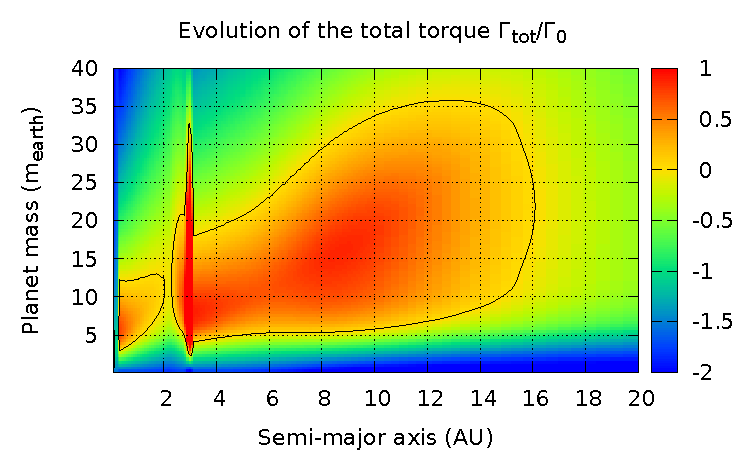
\includegraphics[width=0.49\textwidth]{figure/migration_map/bell_irr.pdf}}\hfill
\subfloat[Sans irradiation]{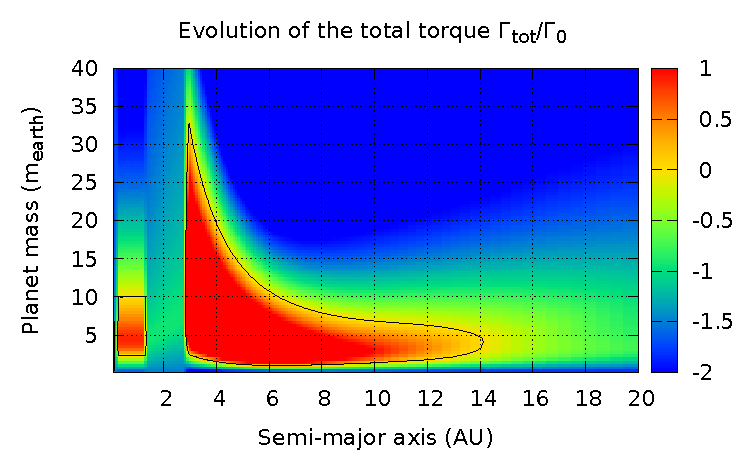
\includegraphics[width=0.49\textwidth]{%
figure/migration_map/bell_noirr.pdf}}

\caption{Influence de l'irradiation sur la carte de migration à travers le profil de température. Afin de visualiser plus
facilement les effets, \cite{bell1994FU} a été utilisé pour l'opacité. \refdisk}\label{fig:irradiation}
\end{figure}

Afin de visualiser l'effet de l'irradiation, nous avons utilisé les lois d'opacités de \cite{bell1994FU}. En effet,
le principal effet de l'irradiation est de lisser le profil de température. Sans irradiation, une transition d'opacité marquée
comme celles de \cite{bell1994FU} se répercute directement sur le profil de température \reffig{fig:temp_profile_irradiation}.
On voit donc apparaître des zone de convergences dues à des transitions d'opacités qui sont déformées par
l'irradiation comme on peut le constater sur \reffig{fig:irradiation}.

\begin{figure}[htb]
\centering
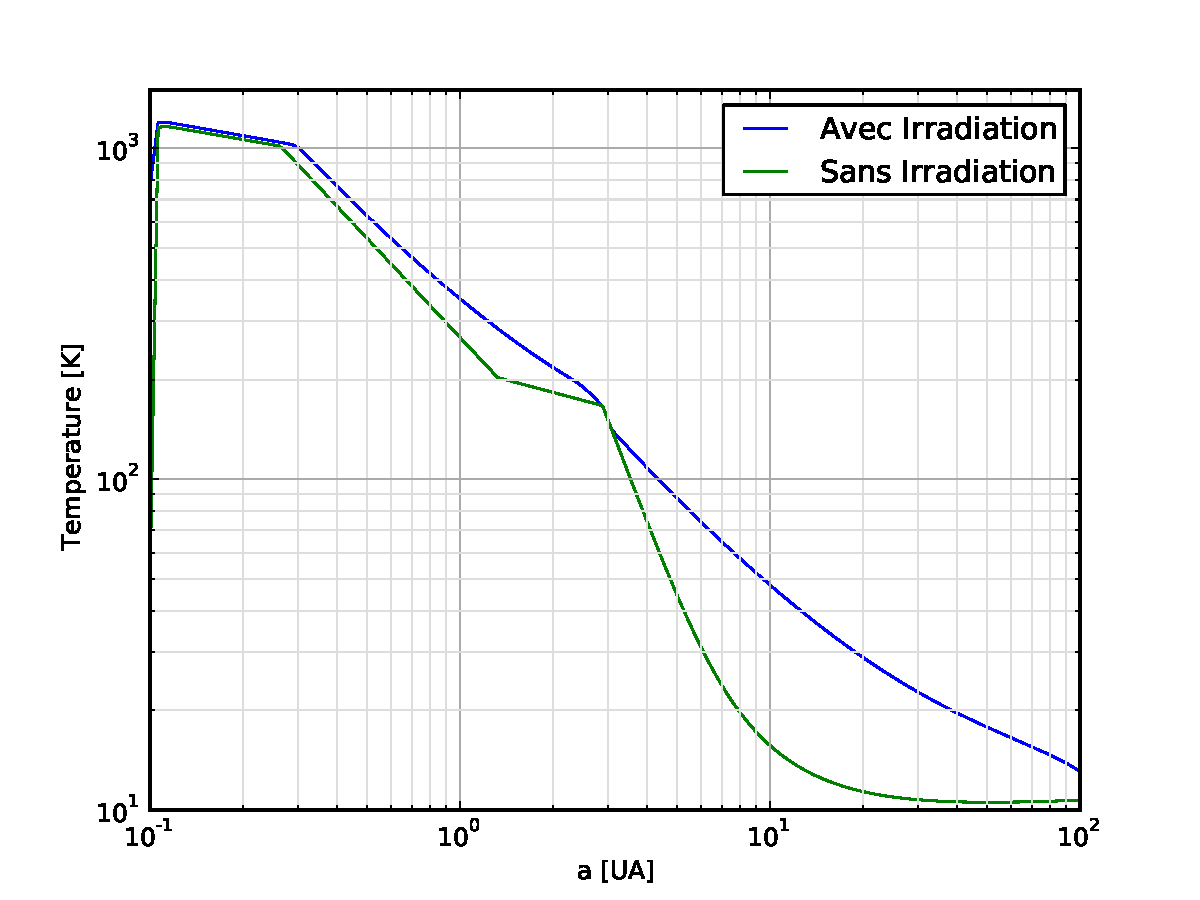
\includegraphics[width=0.6\linewidth]{figure/migration_map/temperature_with_irradiation.pdf}
\caption{Profil de température avec ou sans irradiation. \refdisk}\label{fig:temp_profile_irradiation}
\end{figure}

Ainsi, sans irradiation, les deux transitions d'opacités à $1.3$ et $2.9\unit{UA}$ induisent un changement brutal de la pente
du profil de température, ce qui a pour effet de changer le sens de migration (de positif à négatif, puis l'inverse).

Dans les parties externes, l'irradiation a pour effet de diminuer la pente du profil de température qui tend vers un profil en
$R^{-0.5}$ quand le disque est purement passif.

%TODO expliquer pourquoi les parties externes ``montent'' en masse. En clair, au lieu d'avoir une décroissance de la zone de
% couple nul avec la masse, c'est l'inverse qui se produit quand on active l'irradiation.

%TODO 
\subsection{Table d'opacité}\label{sec:influence_opacity_table}
Le modèle utilisé pour déterminer les opacités dans un disque est bien souvent à peine nommé, et très peu discuté. Pourtant,
l'opacité est une grandeur physique qui a une influence très importante sur la physique du disque et la migration des planètes. 

Dans toute la suite, quand je parlerai de table d'opacité, je désigne le fait d'utiliser un tableau à deux dimensions,
proposant des valeurs de l'opacité pour différentes températures et densités. La table d'opacité est donc définie ici par
opposition à ce que j'appelle des lois d'opacité, modèles dans lesquels l'opacité est définie par des lois de puissance,
fonction de la température et de la densité, dans différents régimes de température et densité.

Ainsi une table d'opacité est simplement une tabulation de l'opacité, alors qu'une loi d'opacité correspond à un ajustement par
une loi de puissance. 

\bigskip

Généralement, c'est la loi d'opacité \cite{bell1994FU} qui est utilisée, aussi bien dans les simulations hydrodynamiques 2D et
3D que dans les simulations N-corps. 

Une autre loi d'opacité existante est \cite{zhu2009nonsteady}, loi quelque peu améliorée par rapport à \cite{bell1994FU},
l'augmentation des capacités des ordinateurs ayant permis de faire des calculs plus précis. 

De plus, nous utilisons aussi le modèle d'opacité très simple décrit par \cite{chambers2009analytic} dans lequel l'opacité est
constante et égale à $\kappa=3$ jusqu'à $1380\unit{K}$ où une transition s'opère vers une loi de puissance. Ce modèle nous
permet de voir l'effet d'un modèle par rapport à un cas où l'opacité est constante. En effet, dans le cas d'un disque
protoplanétaire, seules les régions les plus internes sont susceptibles d'atteindre des températures supérieures à
$1000\unit{K}$. 

Enfin, j'ai souhaité comparer ces deux lois d'opacité avec une table d'opacité, \cite{hure2000transition}. Cette table
d'opacité de Rosseland correspond à la composition suivante $X=0.70$, $Y=0.28$ et $Z=0.02$ et est basée sur
\cite{seaton1994opacities, alexander1994low, henning1996dust}.

\begin{figure}[htb]
\centering
\subfloat[\citep{bell1994FU}]{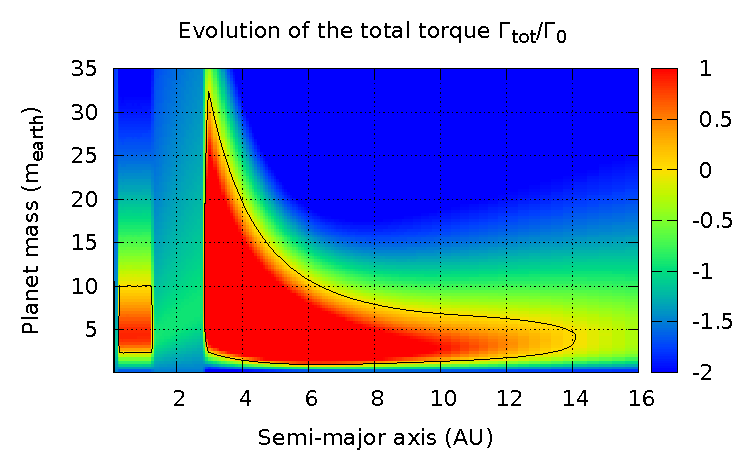
\includegraphics[width=0.49\textwidth]{figure/migration_map/opacity/opacity_bell.pdf}}\hfill
\subfloat[\citep{chambers2009analytic}]{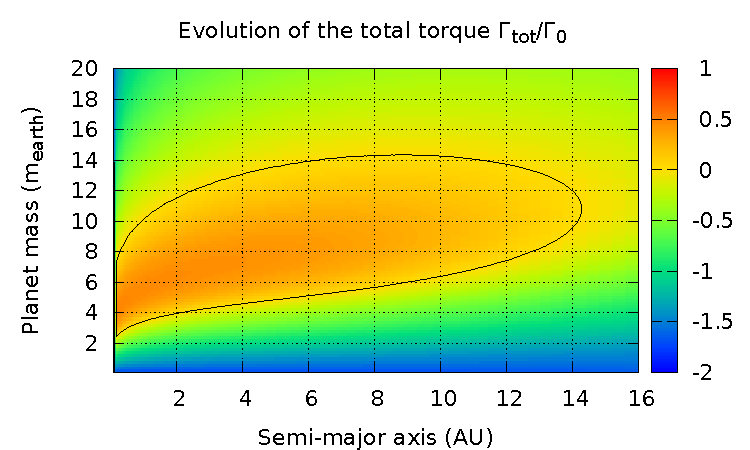
\includegraphics[width=0.49\textwidth]{%
figure/migration_map/opacity/opacity_chambers.pdf}}

\subfloat[\citep{zhu2009nonsteady}]{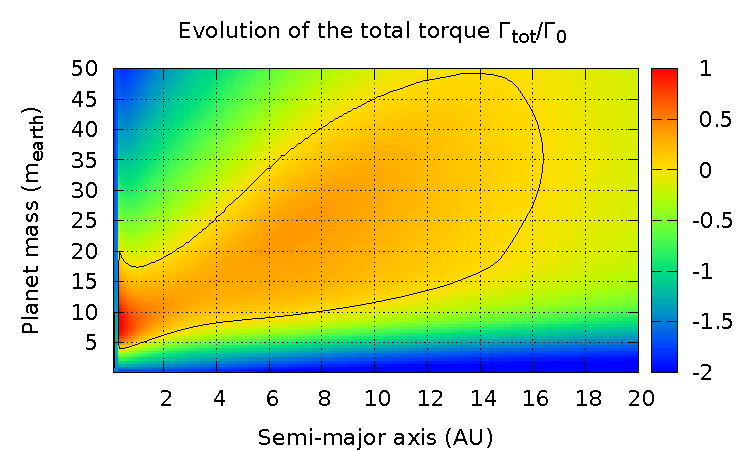
\includegraphics[width=0.49\textwidth]{figure/migration_map/opacity/opacity_zhu.pdf}}\hfill
\subfloat[\citep{hure2000transition}]{\label{fig:opacity_hure}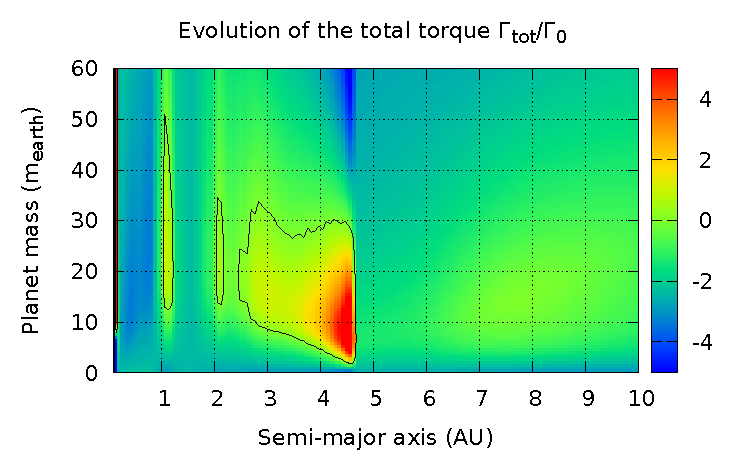
\includegraphics[width=0.49\textwidth]{%
figure/migration_map/opacity/opacity_hure.pdf}}
\caption{Cartes de migration obtenues pour le même disque, mais avec un modèle d'opacité différent. L'irradiation ayant un
effet important sur la carte de migration, elle a été désactivée ici afin de mieux mettre en valeur les différences entre
les modèles d'opacités. Notez que les échelles ne sont pas identiques. \refdisk}
\end{figure}\label{fig:opacity_tables}

\reffig{fig:opacity_tables} montre les différentes cartes de migration que l'on obtient avec le même disque de référence mais
pour les 4 modèles d'opacité considérés. 

On considère la carte avec la table d'opacité \reffig{fig:opacity_hure} comme référence. En effet, les lois d'opacités utilisent
une table d'opacité en amont à partir de laquelle elles déduisent des lois de puissances par morceau afin de reproduire au mieux
la table d'opacité. La table d'opacité se traduit par une carte de migration complexe où chaque aspect de la table se traduit
sur la carte par une variation brutale de la migration. L'opacité a une grande influence sur la migration, que ce soit au
niveau du temps de diffusion qui régi la saturation que vis à vis du profil de température.

L'importance de l'opacité se manifeste au travers du temps de diffusion radiatif. Une opacité plus grande induit un temps de
diffusion radiatif plus important. 

On constate par ailleurs que les lois d'opacité lissent fortement la carte de migration (comparer la carte pour la table
d'opacité d'\cite{hure2000transition} avec les 3 autres). Notons en particulier une transition d'opacité dans \cite{bell1994FU}
qui n'existe pas dans les autres modèles et qui entraine une zone de convergence indépendante de la masse (dans le cas présent
à $1.3\unit{UA}$). Cette transition d'opacité, liée à l'évaporation des grains de glace d'eau, n'est en effet introduite que
dans ce modèle, les autres modèles considérant qu'elle n'illustre aucune réalité physique 
%TODO Ref sur la transition d'opacité fantome

Le modèle d'opacité choisi a donc une grande influence sur la carte de migration et donc le comportement des planètes dans un
disque. À l'heure actuelle, compte tenu de la puissance des ordinateurs, le choix d'une loi d'opacité par rapport à une table
d'opacité ne se justifie plus. En effet, les approximations supplémentaires qu'engendrent une loi d'opacité comparé
à une table brute ne sont pas compensées par le gain de temps de calcul que cela engendre. Dans mon cas, la routine
implémentant la table d'opacité est même plus rapide que la routine pour les lois d'opacités. La seule différence est qu'il
faut stocker un tableau contenant la table d'opacité, ce qui n'est pas limitatif avec les ordinateurs actuels.

Les modèles d'opacités étant une source d'incertitude pour toutes les simulations numériques, que ce soit des simulations
N-corps ou des simulations hydrodynamiques 2D ou 3D, je pense qu'il est important d'apporter une attention particulière au
choix du modèle. 

À l'heure actuelle, dans le cas particulier de la migration planétaire, la valeur de l'opacité ainsi que la pente qu'elle
engendre sur le profil de température sont des sources importantes d'incertitudes. Il pourrait être intéressant de réaliser une
étude d'envergure afin de réaliser une table d'opacité tenant compte des nouvelles capacités des ordinateurs, afin de coller au
mieux à ce que l'on sait des disques. 

Il restera pourtant toujours des incertitudes quant aux propriétés des poussières, taille et quantité, ainsi que son évolution
au cours du temps. La poussière étant une source majeure d'opacité dans le disque, son évolution au cours du temps doit avoir
une influence toute aussi majeure que nous ne pouvons que négliger à l'heure actuelle malgré les implications que cela peut
avoir sur la formation des planètes.

%TODO

\subsection{Longueur de lissage}
Dans les modèles numériques des disques protoplanétaires, le potentiel gravitationnel doit être modifié afin ne pas diverger aux
très faibles distances mutuelles. En particulier, des problèmes peuvent survenir quand on modélise des objets étendus par des
masses ponctuelles. Le modèle de Plummer introduit une longueur de lissage $b$ (souvent notée $b/h$ car sa valeur est exprimée
en fonction de l'échelle de hauteur du disque). la force de gravitation adoucie s'écrit alors : 
\begin{align}
\vect{F_{ij}} &= G m_i m_j \frac{\abs{r_i - r_j}}{\left(\abs{r_i - r_j}^2 + b^2\right)^\sfrac{3}{2}}
\end{align}


De même, dans le cas de simulations hydrodynamiques 2D, le modèle se base sur des moyennes verticales des différentes quantités
physiques. Le lissage du potentiel gravitationnel est ici nécessaire afin de diluer le potentiel et reproduire au mieux l'aspect
3D du disque. On comprend alors aisément que la longueur de lissage va être reliée à l'échelle de hauteur du disque qui est elle
aussi une mesure de l'extension verticale du disque. 

Plusieurs groupes ont cherché à étudier la longueur de lissage en détail, en particulier pour trouver la valeur optimale à
utiliser \citep{hure2009local, muller2012treating}. Ces études cherchent à trouver la longueur de lissage qui permet de
reproduire les simulations 3D à l'aide des simulations 2D. 

Une longueur de lissage relativement importante $b/h = 0.75$ est nécessaire pour reproduire correctement le couple de Lindblad
\citep{masset2002coorbital}. Pour le couple de corotation, la zone fer-à-cheval étant très proche de la planète, ce dernier est
extrêmement sensible à la longueur de lissage. En effet, \cite{masset2002coorbital} a montré que dans certains cas le couple de
corotation pouvait être plus d'un ordre de grandeur plus important en fonction de la valeur du lissage que l'on applique. La
valeur préconisée est alors autour de $b/h\sim 0.5-0.6$. Ainsi, \cite{masset2002coorbital} conclue qu'il est peu probable de
trouver une valeur optimale pour la longueur de lissage, les valeurs optimales pour les couples de Lindblad et de corotation
étant incompatibles. 

\cite{muller2012treating} suggère d'utiliser une longueur de lissage $b/h = 0.7$ tout en notant que des différences notables
subsistent avec les simulations 3D. 

\cite{hure2009local}, en étudiant des disques sans planètes conseillent la plage de valeur suivante $0.13 \lesssim b/h \lesssim
0.29$.

\bigskip

\cite{paardekooper2010torque, paardekooper2011torque} et les formules analytiques ou semi-analytiques qu'ils fournissent pour
décrire la migration de type I (\refeq{eq:lindblad-torque}, \refeq{eq:saturated-corotation-torque},
\refeq{eq:linear-corotation-torque}) introduisent une telle dépendance. 

\begin{figure}[htb]
\centering
\subfloat[$b/h = 0.2$]{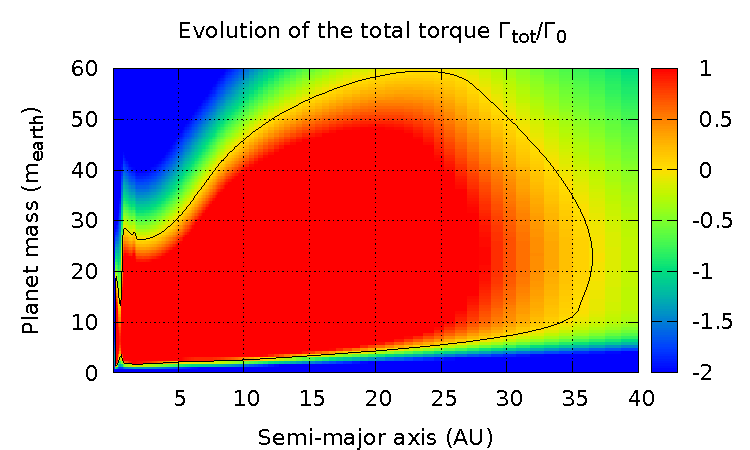
\includegraphics[width=0.49\textwidth]{figure/migration_map/smoothing/smoothing_0_2.pdf}}\hfill
\subfloat[$b/h = 0.4$]{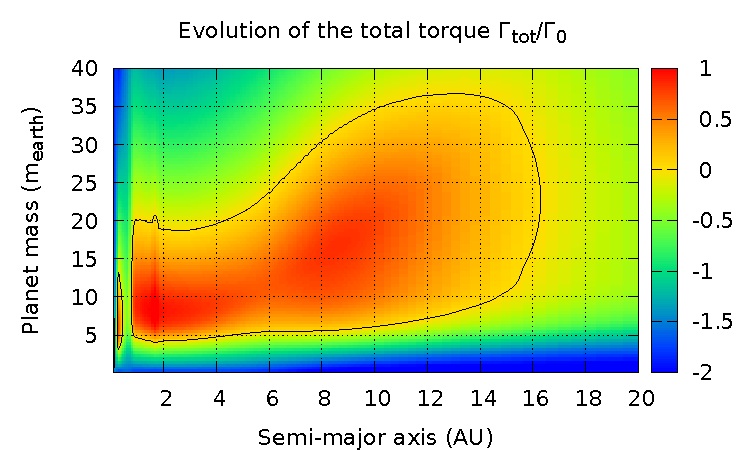
\includegraphics[width=0.49\textwidth]{figure/migration_map/smoothing/smoothing_0_4.pdf}}\\
\subfloat[$b/h = 0.6$]{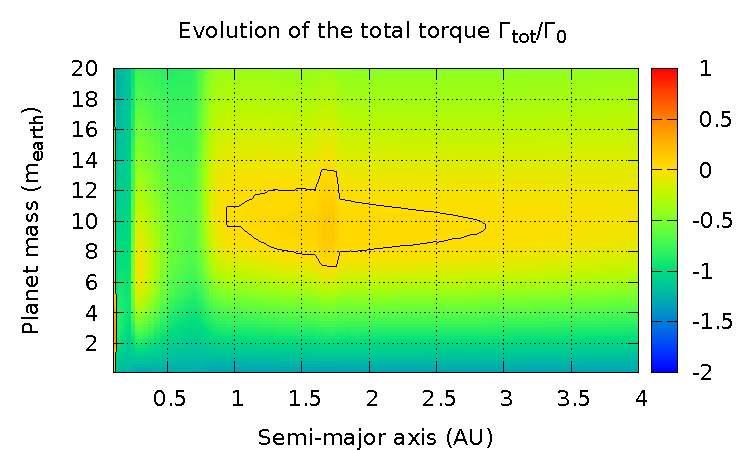
\includegraphics[width=0.49\textwidth]{figure/migration_map/smoothing/smoothing_0_6.pdf}}\hfill
\subfloat[$b/h = 0.7$]{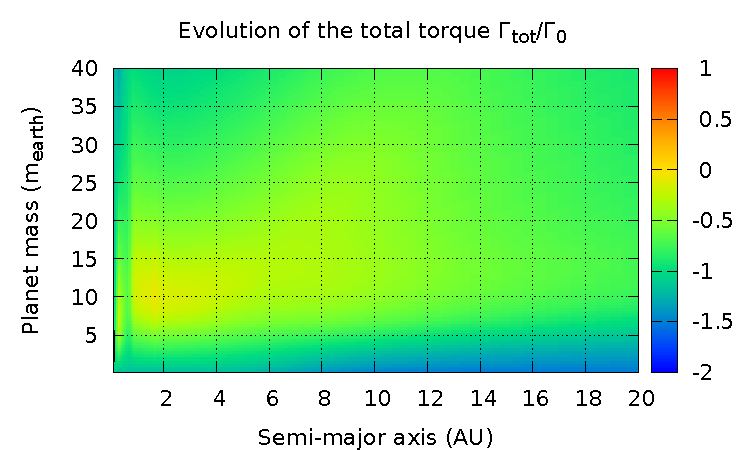
\includegraphics[width=0.49\textwidth]{figure/migration_map/smoothing/smoothing_0_7.pdf}}\\
\caption{Effet de la longueur de lissage $b/h$ du potentiel gravitationnel sur la carte de migration du disque de référence.
\refdisk}\label{fig:migration_map_smoothing}
\end{figure}

\reffig{fig:migration_map_smoothing} montre qu'en fonction de la longueur de lissage, on peut se trouver dans un cas où il y a
migration systématique vers l'intérieur ($b/h=0.7$) ou migration quasi systématique vers l'extérieur ($b/h=0.2$). Si une valeur
de $0.2$ semble peu réaliste au regard de la migration planétaire \citep{muller2012treating}, il est courant de voir des
simulations effectuées avec $b/h=0.3-0.6$ \citep{masset2002coorbital, devalborro2006comparative, paardekooper2009corotation}. 

Une longueur de lissage $0.6 \leqslant b/h \leqslant 0.76$ sous estime le couple de corotation et sur-estime le couple de
Lindblad \citep{masset2002coorbital}. Même si les valeurs préconisées par les études de sensibilités se situent autour de
$0.6-0.7$, les études faisant des simulations hydrodynamiques utilisent plus couramment une valeur de $b/h=0.4$
\citep{paardekooper2011torque}. Il n'existe donc pas de valeur optimale pour la longueur de lissage quand le disque que l'on
modélise est utilisé pour étudier la migration planétaire. Si cette section ne conclue pas quant à une valeur à utiliser pour
$b/h$ c'est avant tout pour insister sur le fait que la seule conclusion à tirer, c'est que la longueur de lissage est une
source importance d'incertitude dans nos modèles. Une longueur de lissage importante (resp. faible) a tendance à favoriser la
migration vers l'intérieur (resp. l'extérieur). 

\begin{figure}[htb]
\centering
\subfloat[$b/h = 0.5$]{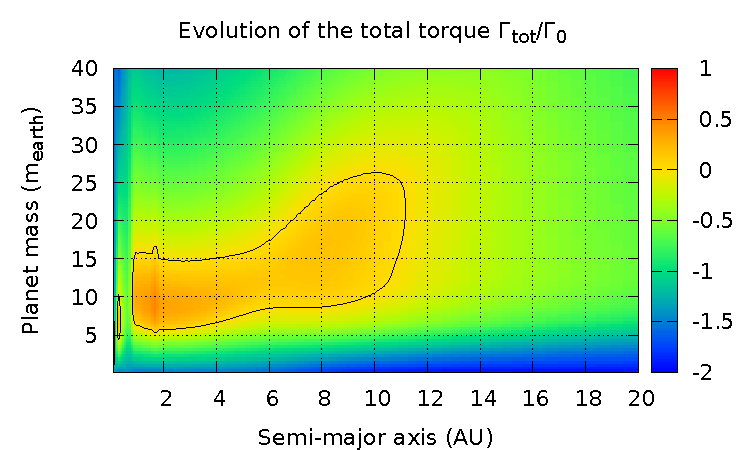
\includegraphics[width=0.49\textwidth]{figure/migration_map/smoothing/smoothing_0_5.pdf}}\hfill
\subfloat[$b/h = 0.76$ pour $\Gamma_L$ et $0.5$ pour
$\Gamma_C$]{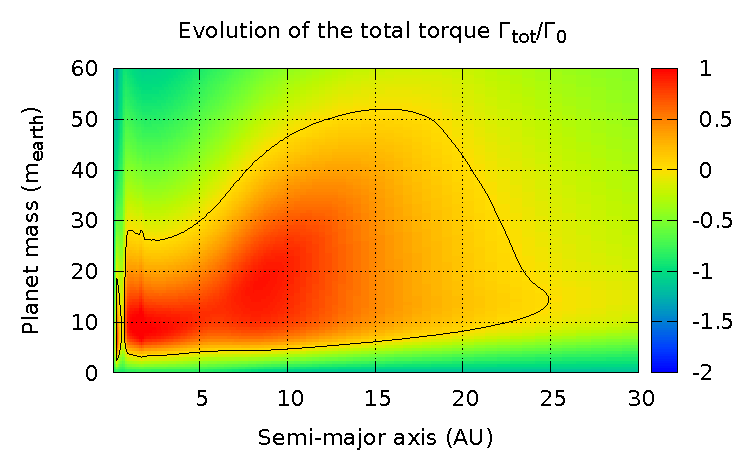
\includegraphics[width=0.49\textwidth]{figure/migration_map/smoothing/smoothing_0_5_modified.pdf}}
\caption{Comparaison d'un cas où la longueur de lissage est fixée à $b/h=0.5$, et d'un autre cas où la longueur de lissage a été
fixée à $0.76$ pour le couple de Lindblad et à $0.5$ pour le couple de Corotation, correspondant aux valeurs conseillées pour
les deux couples séparés \citep{masset2002coorbital}. \refdisk}\label{fig:modified_smoothing}
\end{figure}

Inclure des formules pour la migration de type I nous offre une liberté supplémentaire par rapport aux simulations
hydrodynamique, celle de fixer une longueur de lissage $b/h$ différente pour le couple de Lindblad et pour le couple de
Corotation. Suivant les prescriptions données par \cite{masset2002coorbital} j'ai donc calculé la carte de migration d'une
simulation où je fixe une longueur de lissage $b/h=0.76$ pour le couple de Lindblad, et une longueur de lissage $b/h=0.5$ pour
le couple de Corotation. J'obtiens alors les cartes représentées \reffig{fig:modified_smoothing}, toujours dans le cas du disque
de référence. %TODO décrire le disque de référence en section 3, et en particulier penser à emttre une référence ici vers la
bonne section.

%TODO proposer cette idée d'utiliser une longueur de lissage différente pour lindblad et corotation? En discuter avec Sean et
%Arnaud.


%TODO parler du travail d'audrey? Je voudrais en parler avec elle, lui montrer cette section et savoir ce qu'elle en pense. 
% En particulier, j'aimerais discuter avec elle du fait que la longueur de lissage qu'elle calcule ne peut pas s'appliquer dans
%mon cas à moi. J'aimerais voir si elle saurait m'expliquer pourquoi (dans mon cas j'ai une planète, et pas elle)

\subsection{Masse moléculaire moyenne}
La masse moléculaire moyenne $\mu$ va varier dans le disque, principalement à cause de l'évaporation de certaines
espèces chimiques à différentes températures. La plupart sont négligeable vu leur abondance limitée. Le problème
aurait pu se poser au bord interne du disque, où la température est très importante. Dans cette région là, la masse moléculaire
moyenne peut varier à cause de la photodissociation de la molécule $\mathrm{H_2}$. En supposant que le rapport d'abondance
$\mathrm{He/H}=0.1$, la masse moléculaire, initialement de $\mu=2.35$ passe alors à environ $\mu\sim 1.3$ \citep[Annexe
A]{hure2000transition}.

\begin{figure}[htb]
\centering
\subfloat[$\mu=2.35$]{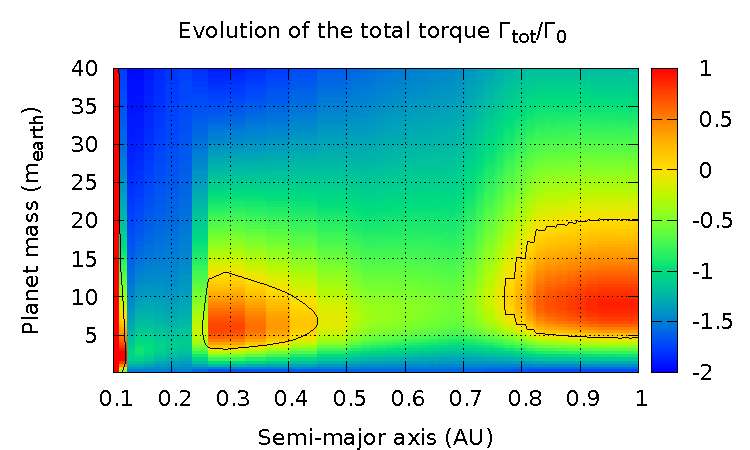
\includegraphics[width=0.49\textwidth]{figure/migration_map/mmw_fully_molecular.pdf}}\hfill
\subfloat[$\mu=1.3$]{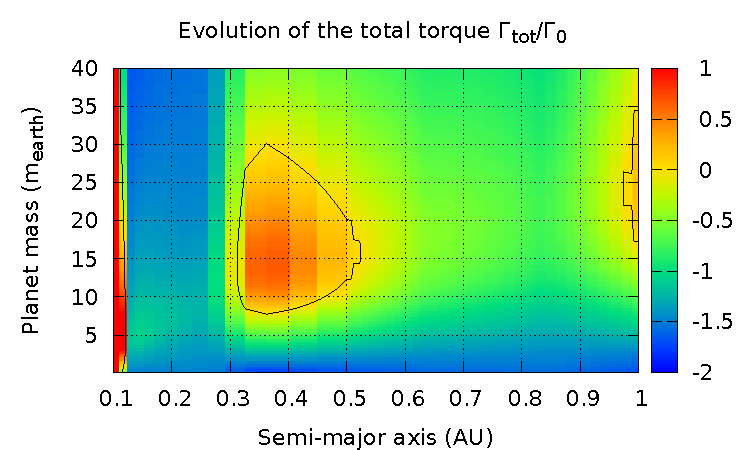
\includegraphics[width=0.49\textwidth]{figure/migration_map/mmw_HI.pdf}}
\caption{Influence de la masse moléculaire moyenne $\mu$ sur la carte de migration. Seules les
parties très internes du disque sont ici représentées. Le même disque est utilisé, seule la masse
moléculaire change afin de refléter l'influence de la photodissociation de $\mathrm{H_2}$ en
$\mathrm{HI}$ quand la température devient importante. \refdisk}\label{fig:migration_map_mmw}
\end{figure}

\reffig{fig:migration_map_mmw} montre l'influence de la masse moléculaire moyenne sur la carte de migration pour un disque
donné. On s'attend à ce que la photodissociation de $\mathrm{H_2}$ ne devienne importante que dans les parties très internes,
bien en dessous de $1\unit{UA}$. Dans ces régions là, on constate que la variation de la masse moléculaire moyenne n'a que peu
d'effet. Il ne nous est donc pas apparu important de prendre cette variation en compte, les changements induits sur la carte de
migration étant bien inférieur à l'influence du modèle d'opacité par exemple. Cet effet nous parait donc négligeable au regard
des incertitudes de notre modèle.